\section{Реализация задачи и решения средствами TLA+ и TLC}

В предыдущих разделах задача верификации соответствия трассы программы и
формальной спецификации была сформулирована как задача разрешимости: по
заданным системе переходов $\mathcal{M} = (X, X_0, R)$, трассе наблюдений
$\tau = (\sigma_1,\dots,\sigma_m)$ и предикату согласованности шага
$C : \Sigma \times X \times X \to \{0,1\}$ требуется определить, существует ли
конечное поведение модели, согласованное с трассой, то есть выполнено ли
условие $\mathrm{B}(\mathcal{M}) \cap \mathrm{M}(\tau) \neq \varnothing$.

В настоящем разделе показывается, каким образом эта математическая постановка
реализуется средствами языка TLA+ и TLC \cite{lamport2002specifying} на примере
спецификации протокола двухфазной транзакции.

\subsection{Общая схема реализации}

Практическая реализация предложенного метода включает следующее:

\begin{enumerate}
    \item \textbf{Спецификация алгоритма.}
    Она задаёт исходную формальную модель проверяемой системы: множество
переменных состояния, начальное условие и отношение переходов
\cite{twophaseimpl}.

    \item \textbf{Спецификация трассы.}
    Она строится поверх базовой спецификации и добавляет ограничения,
порождаемые наблюдаемой трассой выполнения программы \cite{twophaseimpl}.

    \item \textbf{Конфигурация проверки TLC.}
    Она задаёт конкретные значения констант, подключает нужную спецификацию и
определяет условия, при которых трасса считается принятой или отвергнутой
\cite{twophaseimpl}.

    \item \textbf{Библиотека для трассировки программ.}
    Она позволяет формировать трассы выполнения программы и объединять их в
единую трассу при необходимости \cite{tlacimpl}.
\end{enumerate}

\subsection{Соответствие модели и TLA+ спецификации}

С точки зрения математической постановки модель задаётся системой переходов
\[
\mathcal{M} = (X, X_0, R),
\]
где $X$ --- множество состояний, $X_0$ --- множество начальных состояний, а
$R$ --- отношение переходов.

\begin{figure}
  \centering
  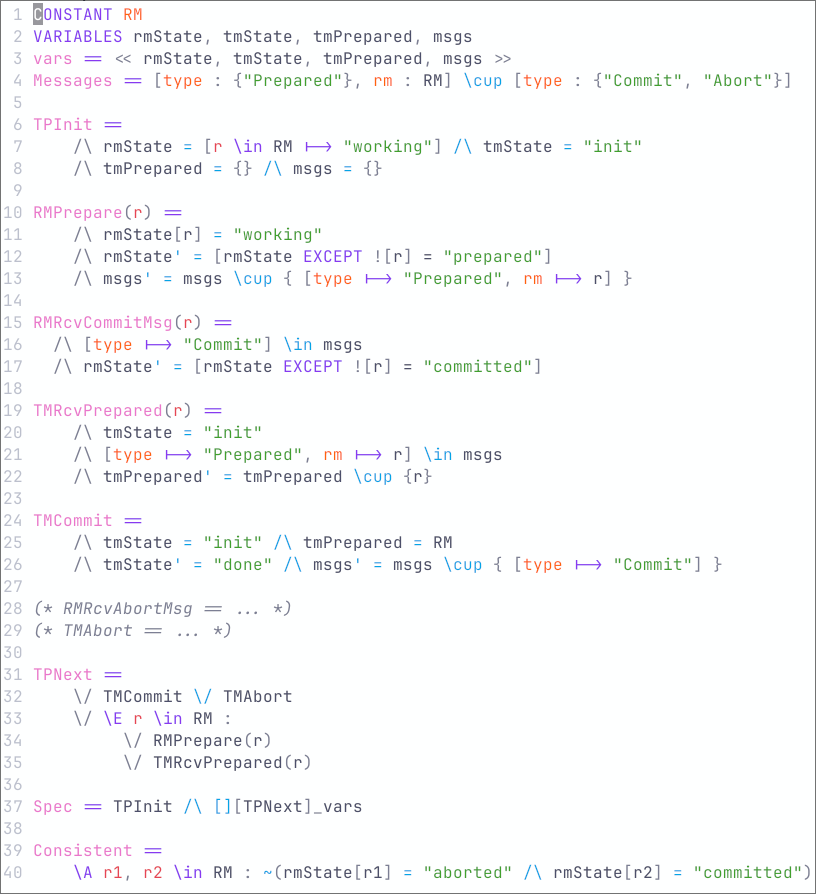
\includegraphics[scale=0.5]{inc/twopc-tla.png}
  \caption{Спецификация алгоритма двухфазной транзакции}
  \label{fig:twopc-tla}
\end{figure}

Для модуля \texttt{TwoPhase} (см. рис. \ref{fig:twopc-tla}) вектор состояния
задаётся переменными
\[
\texttt{vars} = \langle \texttt{rmState}, \texttt{tmState},
\texttt{tmPrepared}, \texttt{msgs} \rangle.
\]
Следовательно, множество $X$ в данном примере можно интерпретировать как
множество всех допустимых значений указанной четвёрки переменных. Начальному
множеству $X_0$ соответствует предикат \texttt{TPInit}, а отношению переходов
$R$ соответствует действие \texttt{TPNext}. Полная спецификация \texttt{Spec}
задаёт множество допустимых бесконечных поведений, однако для цели валидации
трасс существенны только конечные префиксы таких поведений, то есть именно те
объекты, которые в математической постановке были обозначены через
$\mathrm{B}(\mathcal{M})$.

Таким образом, исходная спецификация алгоритма TLA+ задает те самые переходные
системы, которые были введены в математической части.

\subsection{Представление трассы программы}

В математической постановке трасса программы задавалась последовательностью
наблюдений $\tau = (\sigma_1,\sigma_2,\dots,\sigma_m) \in \Sigma^m$.
В рассматриваемой реализации эта последовательность хранится во внешнем файле в
формате NDJSON и считывается оператором \texttt{Trace} (см. рис.
\ref{fig:trace}).

\begin{figure}
  \centering
  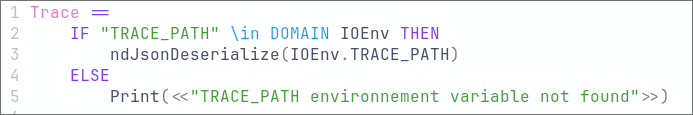
\includegraphics[scale=0.5]{inc/trace.png}
  \caption{Счтывание трассы программы}
  \label{fig:twopc-tla}
\end{figure}

Каждая строка такого файла представляет собой запись, описывающую один шаг
исполнения программы. Запись может содержать имя события, его параметры и набор
частичных обновлений логических переменных модели, пример такой записи
представлен на рис \ref{fig:rm-json}.

\begin{figure}
  \centering
  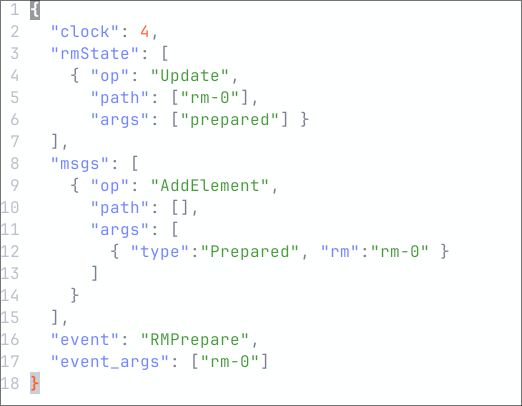
\includegraphics[scale=0.5]{inc/rm-json.png}
  \caption{Пример наблюдения трассы}
  \label{fig:rm-json}
\end{figure}

Тем самым множество наблюдений $\Sigma$ в реализации соответствует множеству
всех допустимых записей трассы данного формата. Последовательность
\texttt{Trace} и есть конкретная реализация трассы $\tau$.

\subsection{Реализация предиката согласованности шага}

Существенным свойством рассматриваемой реализации является синхронность
сопоставления трассы и поведения модели. В математической постановке это
выражено требованием, что каждой записи трассы соответствует ровно один переход
согласованного поведения модели. В реализации это обеспечивается переменной
\texttt{l} и оператором \texttt{IsEvent}, реализация которого представлена на
рис. \ref{fig:is-event}.

\begin{figure}
  \centering
  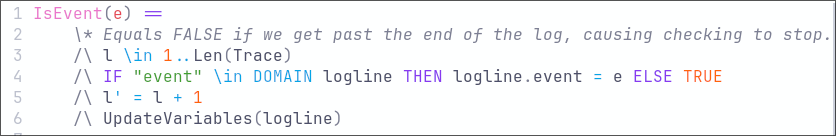
\includegraphics[scale=0.5]{inc/is-event.png}
  \caption{Реализация \texttt{IsEvent}}
  \label{fig:is-event}
\end{figure}

Оператор \texttt{IsEvent(e)} содержит следующие ограничения:
\begin{enumerate}
    \item текущий индекс должен принадлежать диапазону $\texttt{l} \in
1..Len(\texttt{Trace})$;
    \item имя события в текущей записи, если оно задано, должно совпадать с
ожидаемым событием \texttt{e};
    \item после обработки текущей записи индекс увеличивается: $\texttt{l'} =
\texttt{l} + 1$.
\end{enumerate}

Следовательно, каждая успешно обработанная запись трассы продвигает систему на
один шаг вперёд. Это и есть программная реализация условия
\[
\forall i \in \{1,\dots,m\} : C(\sigma_i,x_{i-1},x_i)=1
\]
из математической постановки. Иными словами, в текущем подходе одна запись
трассы соответствует одному переходу ограниченной спецификации. Следует
подчеркнуть, что речь идёт именно о переходе, а не о состоянии. Запись трассы
интерпретируется как ограничение на пару соседних состояний модели.

В математической части предикат $C(\sigma,x,y)$ был введён абстрактно: он
должен принимать значение $1$ тогда и только тогда, когда наблюдение $\sigma$
согласовано с переходом из состояния $x$ в состояние $y$. В TLA+-реализации
этот предикат не задаётся отдельной формулой, а реализуется через сочетание
трёх механизмов (см. рис. \ref{fig:twopc-spec}:
\begin{enumerate}
    \item проверки имени события;
    \item проверки параметров события;
    \item проверки и вычисления значений штрихованных переменных.
\end{enumerate}

\begin{figure}
  \centering
  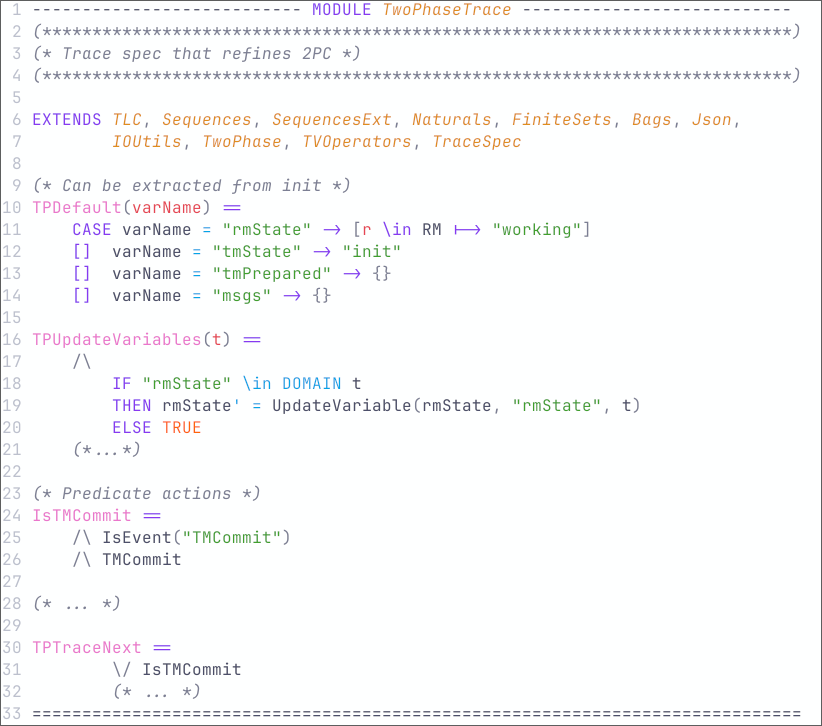
\includegraphics[scale=0.5]{inc/twopc-spec.png}
  \caption{Обертка над спецификацией алгоритма для верификации трасс}
  \label{fig:twopc-spec}
\end{figure}

Проверка имени события реализуется оператором \texttt{IsEvent}, описание
которого приведено выше. Проверка параметров реализуется в действиях вида
\texttt{IsTMCommit}, \texttt{IsRMPrepare}, \texttt{IsRMRcvCommitMsg} и других:
если параметры заданы в трассе, то выбирается соответствующий экземпляр
действия, а если не заданы, то допускается выбор любого допустимого параметра.
Тем самым частичная информация, присутствующая в трассе, корректно
интерпретируется как ограничение на множество допустимых переходов модели.

Проверка обновлений переменных реализуется оператором
\texttt{TPUpdateVariables}. Он анализирует текущую запись трассы и, если для
какой-либо переменной задан список обновлений, вычисляет соответствующее
значение переменной при помощи общего оператора \texttt{ApplyUpdates}. Модуль
\texttt{TVOperators} содержит универсальные операции \texttt{Update},
\texttt{AddElement}, \texttt{RemoveElement}, \texttt{SetKey} и другие, что
позволяет интерпретировать записи трассы как частичные преобразования сложных
структур данных.

Например, если запись трассы фиксирует, что в множество сообщений был добавлен
элемент типа \texttt{Prepared}, а состояние некоторого ресурсного менеджера
изменилось на \texttt{"prepared"}, то \texttt{TPUpdateVariables} накладывает
ровно эти ограничения на значения \texttt{msgs'} и \texttt{rmState'}.
Совместно с действием \texttt{RMPrepare(r)} это даёт точную реализацию условия
согласованности данного наблюдения с переходом модели.

Таким образом, конкретная реализация предиката $C$ зависит от выбранной
спецификации и формата трассы, но общая схема остаётся неизменной:
наблюдение задаёт ограничения на разрешённый шаг модели, а TLC проверяет,
существует ли переход, удовлетворяющий этим ограничениям.

\subsection{Ограниченная спецификация как реализация $\mathrm{M}(\tau)$}

В математической постановке множество $\mathrm{M}(\tau)$ было определено как
множество всех последовательностей состояний, согласованных с трассой.
Средствами TLA+ это множество реализуется неявно через построение
\emph{ограниченной спецификации}, которая разрешает только те шаги, которые
совместимы с текущей записью трассы.

В модуле \texttt{TraceSpec} такая ограниченная спецификация задаётся формулой
\[
\texttt{TraceSpec} \equiv \texttt{TraceInit} \land
[][ \texttt{TraceNext}]_{\langle \texttt{l}, \texttt{Vars} \rangle}.
\]
Здесь \texttt{Vars} обозначает вектор переменных исходной спецификации,
\texttt{BaseInit} --- её начальный предикат, а \texttt{TraceNext} --- дизъюнкция
ограниченных действий, соответствующих шагам исходной модели.

Каждое из действий \texttt{TraceNext} соответствует некоторому действию исходной
спецификации, но дополнительно ограничено текущей записью трассы. Следовательно,
поведения ограниченной спецификации представляют собой ровно те поведения
исходной модели, которые согласованы с данной трассой. Иначе говоря,
ограниченная спецификация реализует множество
\[
\mathrm{B}(\mathcal{M}) \cap \mathrm{M}(\tau).
\]

С практической точки зрения это означает следующее: TLC выполняет обычный
обход пространства состояний, но не всей исходной спецификации, а только той её
части, которая совместима с наблюдаемой трассой. Если соответствующее
пространство состояний непусто, то трасса согласована с моделью; если оно
пусто, то согласованного поведения не существует.

\subsection{Соответствие рекуррентных множеств $D_i$ и работы TLC}

В математическом обосновании решения были введены множества
\[
D_0, D_1, \dots, D_m,
\]
где $D_i$ интерпретировалось как множество всех состояний модели, достижимых
после согласования первых $i$ наблюдений трассы. В реализации на TLC эти
множества не вычисляются явно как отдельные математические объекты, однако
вся процедура обхода ограниченной спецификации фактически эквивалентна именно
такому вычислению.

Действительно, переменная \texttt{l} хранит номер текущей записи трассы.
Начальное состояние ограниченной спецификации соответствует значению
$\texttt{l} = 1$, то есть ещё не обработано ни одной записи трассы. После
обработки первой записи получаются состояния со значением $\texttt{l} = 2$,
после обработки второй --- со значением $\texttt{l} = 3$, и так далее. Поэтому
множество всех достижимых состояний ограниченной спецификации с фиксированным
значением
\[
\texttt{l} = i+1
\]
естественно соответствует множеству $D_i$ из математической постановки.

Иначе говоря, TLC реализует пошаговое построение множеств $D_i$ не в явном
формульном виде, а через стандартный перебор достижимых состояний ограниченной
спецификации. Это и есть алгоритмическая интерпретация доказанного в предыдущем
разделе критерия $D_m \neq \varnothing$.

\subsection{Критерий успешной проверки в TLC}

В математической постановке критерий согласованности был выражен условием
$\mathrm{B}(\mathcal{M}) \cap \mathrm{M}(\tau) \neq \varnothing$, а в разделе
обоснования решения было показано, что этот критерий эквивалентен условию $D_m
\neq \varnothing$. В реализации на TLC данная идея выражается через постусловие
\texttt{TraceAccepted}.

\begin{figure}
  \centering
  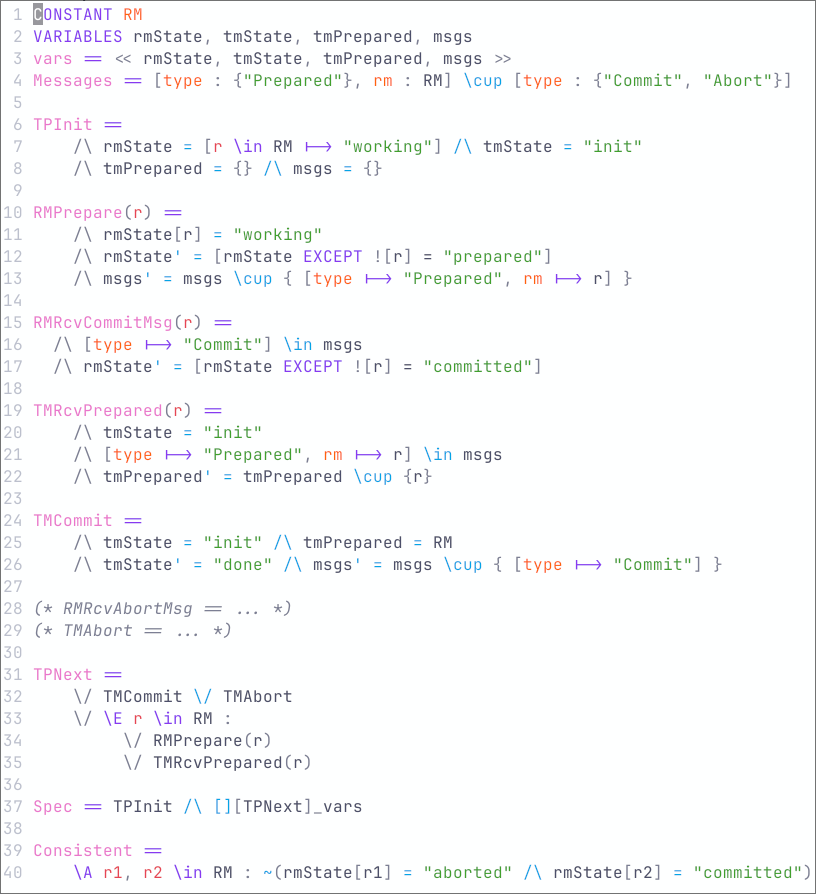
\includegraphics[scale=0.5]{inc/twopc-tla.png}
  \caption{Реализация \texttt{TraceAccepted}}
  \label{fig:twopc-tla}
\end{figure}

Оператор \texttt{TraceAccepted} использует статистику TLC и проверяет, что
диаметр построенного ограниченного пространства состояний совпадает с длиной
трассы с точностью до единицы. Содержательно это означает, что TLC удалось
построить путь, последовательно согласующий все записи трассы. Если же такой
путь отсутствует, то значение \texttt{TraceAccepted} ложно, и проверка
завершается сообщением об ошибке.

Использование диаметра здесь оправдано структурой ограниченной спецификации:
при каждом шаге переменная \texttt{l} увеличивается на единицу, поэтому обход
пространства состояний естественным образом организован по уровням,
соответствующим длине уже согласованного префикса трассы. Следовательно,
достижение последнего уровня эквивалентно существованию согласованного
поведения полной длины.

\subsection{Особенности и ограничения рассматриваемой реализации}

Следует отметить, что реализованная схема соответствует той математической
постановке, которая была принята в работе, а именно синхронному сопоставлению
трассы и поведения модели. Каждой записи трассы соответствует ровно один
переход ограниченной спецификации. Это упрощает как математическое описание,
так и программную реализацию.

Вместе с тем структура модулей показывает, что возможны и более общие
расширения. В частности, в коде предусмотрены заготовки для обработки
stuttering-переходов и для задания композиции действий, однако в текущем
варианте они отключены. Следовательно, реализованное решение охватывает тот
класс задач, в котором инструментированная трасса уже приведена к уровню
атомарности, совместимому с шагами спецификации.

Ещё одно ограничение связано с неполнотой трассы. Если записи трассы содержат
слишком мало информации, то множество допустимых интерпретаций отдельного шага
становится слишком широким. Тогда TLC может найти некоторое согласованное
поведение модели, хотя фактическое поведение программы восстановлено по трассе
неоднозначно. Таким образом, практическая точность метода зависит не только от
корректности спецификации, но и от качества инструментирования кода и полноты
логируемых данных.
